%% -*- mode: latex; mode: reftex; mode: flyspell; TeX-master: "top.tex"; -*-

The  process  of forming  functional  connections  between neurons  is
complex  and   dynamic.   Time-lapse  microscopy   has  revealed  that
differentiating  neurons undergo  a large  range of  dynamic processes
including cell body motility, filopodial dynamics, and repeated cycles
of  neurite growth  and  retraction.  Of  critical  importance is  the
process  by which  axons and  dendrites are  formed in  which a neurite
ceases retracting, extends a   long  distance, and eventually  forms
a connection. These  dynamic events are  governed by a  complex protein
network that  coordinates  cellular  dynamic functions 
within the cytoskeleton, membrane, etc.

%including
%cytoskeletal, adhesion, and membrane trafficking dynamics.


%----------------------------------------------------------------------------
\begin{figure}[t]
  %\begin{center}
  \centering
       \begin{tabular}{@{}c@{}|c@{}}
        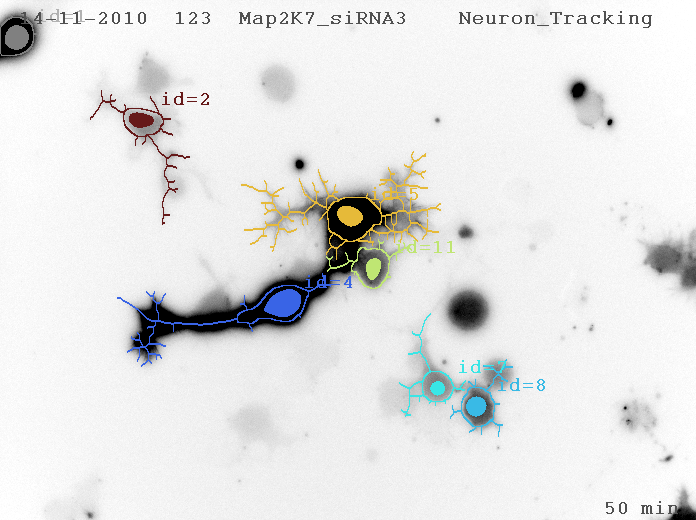
\includegraphics[width=62mm] {images/mv1_005.png}  &
        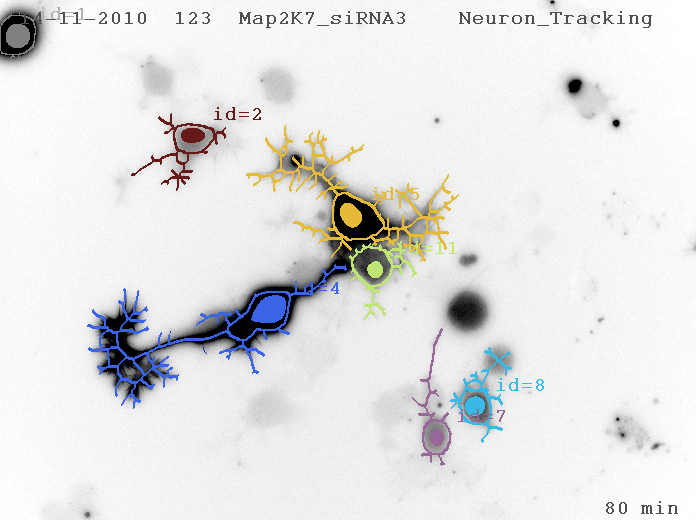
\includegraphics[width=62mm] {images/mv1_008.png} \\ [-1ex]
        \hline \\ [-2.8ex]
        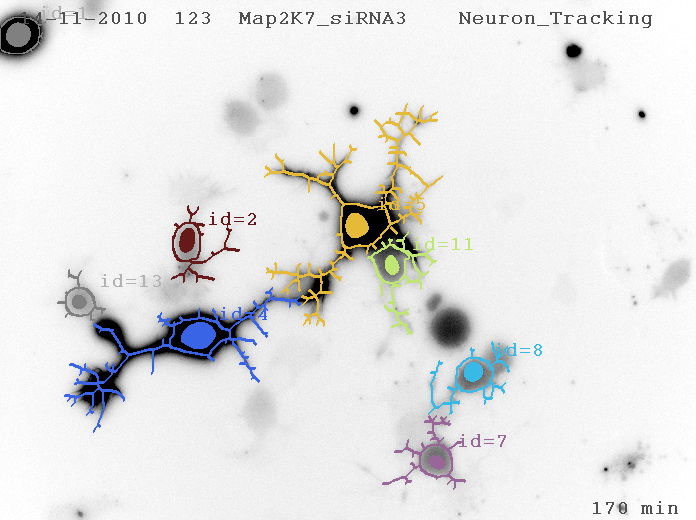
\includegraphics[width=62mm] {images/mv1_017.png}  &
        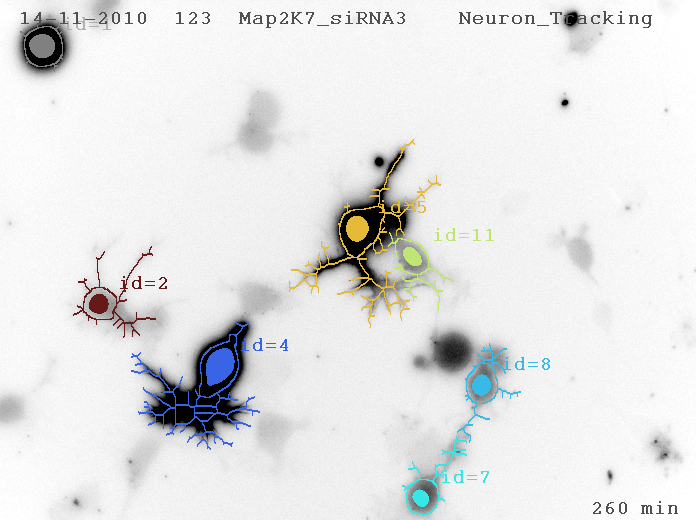
\includegraphics[width=62mm] {images/mv1_026.png} \\ [-1ex]
        \hline \\ [-3.1ex]
       \end{tabular} 
       
      \begin{tabular}{@{}c@{}c@{}c@{}c@{}}
        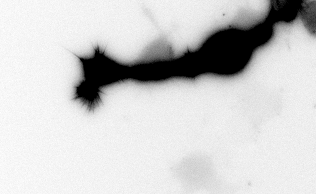
\includegraphics[width=31mm] {images/0_005.png} &
        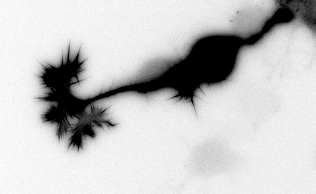
\includegraphics[width=31mm] {images/0_008.png} & 
        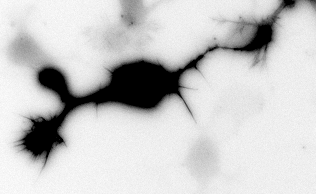
\includegraphics[width=31mm] {images/0_017.png} & 
        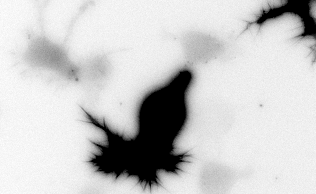
\includegraphics[width=31mm] {images/0_026.png} \\ [-1ex]
        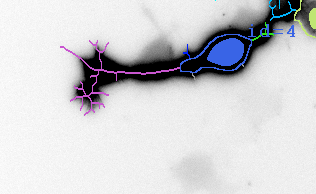
\includegraphics[width=31mm] {images/2_005.png} &
        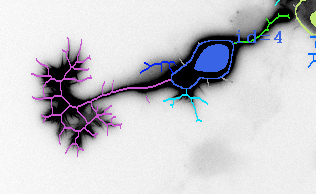
\includegraphics[width=31mm] {images/2_008.png} & 
        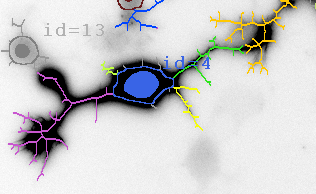
\includegraphics[width=31mm] {images/2_017.png} & 
        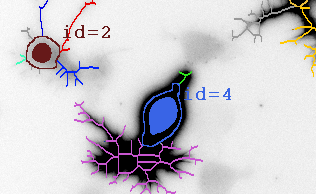
\includegraphics[width=31mm] {images/2_026.png} \\ [-1ex]
        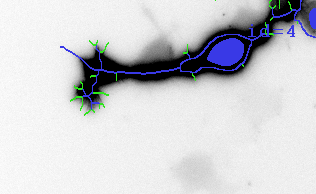
\includegraphics[width=31mm] {images/3_005.png} &
        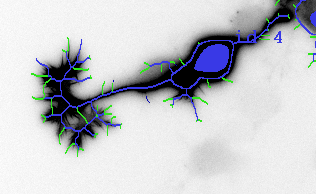
\includegraphics[width=31mm] {images/3_008.png} & 
        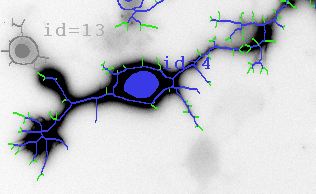
\includegraphics[width=31mm] {images/3_017.png} & 
        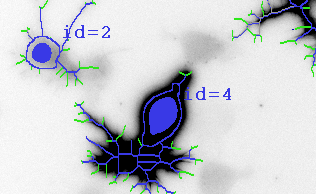
\includegraphics[width=31mm] {images/3_026.png} \\ [-3.5ex]
        {\footnotesize $t = 50$ min} & 
        {\footnotesize $t = 80$ min} & 
        {\footnotesize $t = 170$ min} & 
        {\footnotesize $t = 260$ min} \\ [-1ex]
      \end{tabular}
    \vspace{-2mm}  
    \caption{ {\footnotesize {\it Neuron  Tracking Results.  } The top
        two rows  contain frames from an experiment  where MAP2K7 gene
        functions are inhibited.  For visibility we enhanced the image
        contrast.  Tracked neurons are marked by a unique color and id
        tag.   Nuclei  are denoted  by  filled  ellipsoids, somata  as
        contours,  and neurites  as trees.   Bottom rows  show details
        from  above: 1)  enhanced original  image 2)  tracked neurites
        marked with a different colors 3) detected filopodia marked in
        green.   Our  approach   performs  well  even  in  challenging
        situations where neurons appear in close proximity. Videos are
        provided  in supplementary  materials.  Note: faintly  stained
        cells are ignored for robustness.}}
    \label{fig:video}
 % \end{center}
\end{figure}
%% by linking nucleus detections  and ``growing'' the
%%         neuron from the nucleus seed
%----------------------------------------------------------------------------

 %% Extremely  faint cells  are not
 %%        tracked  due to  the  issues in  the  staining process.

Recently, powerful tools have become available to help investigate the
molecular   interactions  that   govern  such   complex  morphogenetic
processes  at  the systems  biology  level.   RNA interference  (RNAi)
technology,  fluorescent  protein   labeling,  image  processing,  and
automated high-throughput  microscopy have  opened the door  for large
scale  perturbation studies. RNAi  screens have  already led  to novel
insights   into  a  number   of  cellular   processes  such   as  cell
migration~\cite{Bakal07}  and endocytosis~\cite{Collinet10}.  However,
limitations  in  image  processing  technology  have  restricted  most
studies to steady-state analysis using single images.

%These experiments are, in principle, capable of quantifying morphology
%and dynamics at the single cell level.

%% To have a clear understanding of this complex process, knowledge of
%% the dynamics of the neurites is essential.
%% cycles of neurite extrusion, retraction, and branching that are critical to de-
%% velopment []
%% Neurites
%% emanating from the soma undergo

%% High-throughput RNAi  screens have already  led to important  steps in
%% our  understanding  of  neuronal  development and  function.  OLIVIER,
%% PLEASE HELP US OUT WITH  SOME EXAMPLES HERE! INCLUDE SOME IMAGE-BASED,
%% AND  SOME THAT  USE  OTHER  METHODS. However,  due  to limitations  in
%% technology,  most studies  are  limited to  either steady-state  image
%% analysis, or focus on the functions of a single gene.

Knowledge  of dynamics is  essential if we are  to understand
complex  processes such  as neuron  morphogenesis.  However, designing
algorithms to quantify dynamic  behaviors is challenging, and
automatic methods  have appeared only  very recently. State-of-the-art
high-throughput techniques have successfully quantified morphodynamics
of  HeLA cancer  cells  in an  effort  to understand  the process  of
mitosis~\cite{Held10,Neumann10,Zhu05}.   However,  the morphology  and
dynamics of  these cell types  are relatively simple in  comparison to
the wide range of morphodynamics exhibited by differentiating neurons.


%% This  is  unfortunate,  because  the  process  of  forming  functional
%% connections   between  neurons   is  extremely   dynamic.   Time-lapse
%% microscopy   has  revealed  complex   cycles  of   neurite  extrusion,
%% retraction,  and branching that  are critical  to development~\cite{}.
%% While steady-state  image analysis  has expanded our  understanding of
%% morphogenesis~\cite{}, it  can not provide a complete  picture of this
%% process.  Neurites emanating from  the soma undergo repeated cycles of
%% growth and retraction during which the morphology can range from short
%% star-like highly  bifurcated trees  to very elongated  structures with
%% few bifurcations, as can be seen in Figure~\ref{}.  At some point, one
%% process stops  retracting and  extends, eventually becoming  the axon,
%% while  other  processes continue  to  extend  and retract,  eventually
%% becoming  dendrites. To  have a  clear understanding  of  this complex
%% process,  knowledge of  the  dynamics of  the  neurites is  essential.
%% However, designing algorithms to quantify these behaviors is extremely
%% challenging and until very recently, automatic methods to quantify and
%% analyze   cellular   dynamics    did   not   exist~\cite{}.    Several
%% state-of-the-art high-throughput techniques have quantified morphology
%% and  dynamics for  HeLA cancer  cells~\cite{Held10,Neumann10,Zhu05} as
%% well as for {\it Caenorhabditis elegans}~\cite{Sonnichsen05}. However,
%% the morphology and dynamics of  these cell types are relatively simple
%% in comparison to  the wide range of dynamics  and morphology exhibited
%% by developing neurons.

%exhibit much less complex  dynamics and morphologies
%than developing neurons.
 
We  propose a  fully  automatic method  for  detecting, tracking,  and
segmenting the  entire neuron  including the nucleus,  soma, neurites,
and filopodia. We begin by  detecting nuclei in each time step.  Next,
a greedy  tracking algorithm  associates detected nuclei  in different
time steps,  forming lists  of detections corresponding  to individual
neurons.  Using  the detected nuclei as seed  points, a region-growing
algorithm segments the soma of  each neuron.  The somata are used to
initialize a joint segmentation of the entire structure of all neurons
appearing in  a image using  a probabilistic method based  on shortest
path computations.   We extract a  graph describing the  morphology of
the  neurites from  the segmentation.   The greedy  tracking algorithm
also tracks individual neurites  over time, and filopodia are detected
by analyzing the topology of each neurite.



%Filopodia are detected by analyzing the topology of the graph.
%% The greedy tracking algorithm and 

%% Our contribution of 

%% put together a system that can perform
%% statistical analysis on videos in a way that nobody has done before.
%% It is efficient and works on a large scale. We analyzed 560 videos in
%% the matter of a few hours. And we used it to confirm known results and
%% make new statistical observations that biologists could not do before

%   Finally,
%filopodia  are  detected  by  analyzing  the topology  of  the  graph
%corresponding to each neurite.

As   demonstrated  in   Fig.~\ref{fig:video}  and   our  supplementary
materials, our  approach produces reliable  segmentations that capture
complex  neuron  dynamics.   For   validation,  we  applied  it  to  a
small-scale  siRNA screen  of 5  genes (3  siRNAs/gene).  Steady-state
phenotypes  associated with  these genes  were previously  analyzed in
MetaMorph\texttrademark~\cite{Pertz08} with simple image measurements.
In addition, a few  dynamic phenotypes were qualitatively observed but
not quantified.  Quantitative analysis  of features extracted from our
segmentations  confirms the  effects  described in~\cite{Pertz08},  as
well as  the observed dynamic behaviors.  Our  analysis also uncovered
new dynamic behaviors which were previously unquantifiable.


While  our greedy tracking  and probabilistic  segmentation algorithms
are  novel,  they are designed to be efficient and thus are relatively 
simple.  The  main contribution of this  paper is the  system as a
whole,  which  is capable  of  high-throughput  processing of  videos,
tracking individual  parts of  neurons, and quantifying  their dynamic
behaviors in ways that were previously not possible.


%%   In
%% particular,  loss  of function  of  the  MAP2K7  gene resulted  in  an
%% increased number of  neurites per cell, but the  neurites were shorter
%% than  in the control.   RHOA loss  of function  resulted in  fewer but
%% longer neurites, with  a reduced number of filopodia.   SRGAP2 loss of
%% function showed longer neurite length and an increase in the number of
%% filopodia.  Additionally, we have observed new dynamic behaviors, such
%% as ({\it we will pick the most interesting things tonight!!!!!!!!}).

% in a  neuronal-like  NE-115 model  cell system.

%%   We  begin  by  detecting
%% H2B-mcherry  chromatin  marked  nuclei  in  each time  stop  based  on
%% fluorescence [OLIVIER  HELP HERE]. 


%%  For that purpose, we are  taking an RNA interference approach in which
%% each of  the 220  candidate genes of  the network mentioned  above are
%% knocked  down in  a  neuronal-like N1E-115  model  cell system  (three
%% different  siRNAs  per  target).   In  this  experiment,  the  F-actin
%% cytoskeleton and the nucleus of the cells are labeled in two different
%% colors by expression of genetically-encoded probes that take advantage
%% of green fluorescent protein  technology.

%% We have analyzed $420$ video sequences I  NEED TO KNOW WHAT EXACTLY ARE WE DOING
%% under different  gene combinations. By using  our system, we  have found similar
%% effects as  described in CITEOLIVIER. By  knocking down the  {\it Map2kT} gene,
%% the  neurons  show  a  higher  number  of shorter  neurites  thant  the  control
%% experiment. By  knocking down the {\it  Rhoa} gene, the neurites  are longer and
%% the  philopodia mass  decreases. Such  effects corroborate  the validity  of our
%% measurements. We have observed other behaviours,  such as ({\it we will pick the
%%   most interesting things tonight}).


%robust, but computationally efficient.

%% Our  method for  neuron tracking  and  segmentation consitsts  of the  following
%% steps. First,  we detect nuclei  at each frame  based on their  fluroescence. We
%% associate  nuclei among consecutive  frames using  a greedy  tracking algorithm.
%% Each nucleus is then grown to form  a soma.  Using such somas as initial points,
%% the whole  neurons are  segmented using  a novel method  based on  shortest path
%% computations.  From each segmentation we form the neuronal tree.  From each tree
%% we infer the  individual neurites. For each neuron, its  neurites are tracked to
%% analyze their  individual dynamics.  Finally,  we detect filopodia  by analyzing
%% the graph structure of each neurite.



%% % 20110308 gg - complex neuronal shape
%% Neurons show a wide range of morphology and dynamics.  Their structure
%% range from star-like highly bifurcated  trees to ellongated structures with just
%% few  bifurcations.  Neurons  and  neurites protrude  and  collapse at  different
%% frequencies Furthermore, the dynamics of  growth cones can vary drastically from
%% the dynamics of neurites.  Designing  algorithms to extract statistics from such
%% complex systems is extremely challenging.



%% % 20110308 gg - we are the ones to combine tracking and tree tracing
%% While many methods for tracking and tree inference of neurons exist, they either
%% perform the  former or  the latter. We  present the  first method that  not only
%% tracks the  position of the neurons,  but also tracks temporal  changes in their
%% morphology. This allows us to  obtain statistical measures at differernt levels.
%% We can  infer both the  evolution of neurons,  and of individual  neurites across
%% time.








\comment{
FURTHER OUTLINE:
\begin{itemize}
\item  discuss a little bit about why neurons / neurites are harder than these other cells

\item  add a few more points about the advantages of dynamic analysis over static

\item give a detailed outline of our approach

\item list the benefits and novelties of our approach

\item discuss our findings from the results section (our validation of known results in addition to new findings)
\end{itemize}
}

%% However, even  though it  is now possible  to efficiently  image large
%% volumes of dynamic processes in  living cells and tissues, research is
%% still limited by a lack of  tools to analyze the massive datasets that
%% are  typically   generated  in   such  experiments.  In   most  cases,
%% biologically relevant  features must be  extracted by hand  or through
%% simple  image processing  techniques, limiting  research  to anecdotal
%% rather  than  statistical  evidence.  In  the  worst  case,  important
%% behaviors which cannot be discerned by human observers are overlooked.
%% Thus, there is  a great need for generalized  computational methods to
%% perform   automatic,  unbiased   quantitative   analyses  of   dynamic
%% microscopic images.







%% Proper   functioning  of  the   nervous  system   requires  functional
%% connections  between   neurons  and  their   targets.   This  requires
%% undifferentiated cells to expand  cylindrical extensions with a growth
%% cone at its distal tip in  a process called neurite outgrowth. In this
%% process,  the round  shape of  the  cell is  broken down  and a  small
%% extension is generated.The latter  will subsequently elongate to build
%% proper neurite. Timelapse microscopy studies show that this process is
%% intrinsically  dynamic  and highly  complex,  with  cycles of  neurite
%% protrusion, retraction and  branching. Mostly due to the  state of the
%% technology,  two  factors  limit  the understanding  of  this  complex
%% process: 1.  Most studies  focusing on neurite  growth have  only used
%% “static”  snapshots  of the  process,  and  thus  ignored the  complex
%% morphodynamics inherent  to that system.   2. Most studies  on neurite
%% outgrowth  have focused  on  only one  gene  at a  time precluding  an
%% holistic, systems  view of how  multiple components integrate  to fine
%% tune this  complex morphodynamic process. Here, we  propose to address
%% these  two concerns  by performing  a large  scale  perturbation study
%% using the neurite morphodynamics as a readout.

%% For that purpose, we are  taking an RNA interference approach in which
%% each of  the 220  candidate genes of  the network mentioned  above are
%% knocked  down in  a  neuronal-like N1E-115  model  cell system  (three
%% different  siRNAs  per  target).   In  this  experiment,  the  F-actin
%% cytoskeleton and the nucleus of the cells are labeled in two different
%% colors by expression of genetically-encoded probes that take advantage
%% of green fluorescent protein  technology. This allows to visualize the
%% dynamics  of  these two  organelles  in  single  living cells.   Using
%% high-throughput  microscopy,  we  are  in the  process  of  generating
%% timelapse datasets in which the neurite and nucleus morphodynamics are
%% monitored  during   the  whole   neurite  outgrowth  process   in  the
%% unperturbed and perturbed states. This requires the acquisition of 660
%% perturbation  experiments  in  which  10 timelapse  datasets  will  be
%% acquired  each  time, leading  to  the  production  of 6600  timelapse
%% movies.  This  hight  volume  of  data  requires  both  the  automatic
%% segmentation  of  the different  cellular  structures  as  well as  an
%% efficient  statistical  pipeline  to  analyze the  complexity  of  the
%% morphodynamic features we want to extract.
